\documentclass[oneside,11pt,letter]{article}

% General include (DO NOT MODIFY)
\include{cs446include}

%%%%%%%%%%%%%%%%%%%%%%
%CHANGE
%.   to booklet to print the problems only
%
%    to both to print problems and solutions
%%%%%%%%%%%%%%%%%%%%%%

\newcommand{\type}{booklet}
%\newcommand{\type}{both}

% Custom adjustments (CHANGE THIS FILE FOR ADDITIONAL ADJUSTMENTS)
\include{cs446custom}

%************************************************************************
%                                                                       *
%            End of preamble and beginning of text.                     *
%                                                                       *
%************************************************************************

\begin{document}
%------------------------- Title Page ----------------------------------
\thispagestyle{empty}
\baselineskip2.5ex
{\bf University of Illinois}
\hfill
Spring 2018

{\Large
\begin{center}
{\sf CS\,446: Machine Learning}\\ Homework 7\\
\end{center}
}
{\large
\begin{center}
{\color{red}Due on Tuesday, March 6, 2018, 11:59 a.m. Central Time}
\end{center}
}



\ifthenelse{\equal{\type}{booklet}}{
\newcommand{\MRFStudSolAA}{
$$
\text{\#configurations} = 5^4 = 625
$$
}
\newcommand{\MRFStudSolAB}{
No, because the graph is cyclic, implying the graph cannot be\\represented as a dependency tree.
}
\newcommand{\MRFStudSolAC}{
$\text{\#messages} = \|\lambda\_{p,r,y_r}\|$; where p is the number of parents 4, r is\\the number of regions 8 and $y_r$ is the number of labels 5.
$\text{\#messages} = 4*5*8 = 160$
}
\newcommand{\MRFStudSolBA}{
\begin{align*}
\text{define}\quad& r \in \{\{1\}, \{2\}, \{1,2\}\}\\
& x_1 \in \{0,1\}\\
& x_2 \in \{0,1\}\\
& x_{1,2} \in \{(0,0), (0,1), (1,0), (1,1)\}\\
\\
\text{maximize}\quad&
\begin{bmatrix}b_1(0)\\b_1(1)\\b_2(0)\\b_2(1)\\b_{1,2}(0,0)\\b_{1,2}(0,1)\\b_{1,2}(1,0)\\b_{1,2}(1,1)\end{bmatrix}^T\begin{bmatrix}1\\2\\1\\2\\-1\\2\\-1\\-1\end{bmatrix}\\
\\
\text{subject to}\quad& b_r(x_r) \in \{0,1\} \quad r\\
&\sum_{x_1}b_1(x_1)  = 1\\
&\sum_{x_2}b_1(x_2)  = 1\\
&\sum_{x_{1,2}}b_{1,2}(x_{1,2})  = 1\\
& b_{1,2}(0,0) + b_{1,2}(0,1) = b_1(0) \\
& b_{1,2}(1,0) + b_{1,2}(1,1) = b_1(1) \\
& b_{1,2}(0,0) + b_{1,2}(1,0) = b_2(0) \\
& b_{1,2}(0,1) + b_{1,2}(1,1) = b_2(1) \\
\end{align*}}

\newcommand{\MRFStudSolBB}{
$$
\mathbf{b} = \begin{bmatrix}b_1(0)\\b_1(1)\\b_2(0)\\b_2(1)\\b_{1,2}(0,0)\\b_{1,2}(0,1)\\b_{1,2}(1,0)\\b_{1,2}(1,1)\end{bmatrix}
=
\begin{bmatrix}1\\0\\0\\1\\0\\1\\0\\0\end{bmatrix}
$$

$$
\mathbf{b}^T\theta(\mathbf{x}) = 5
$$
}

\newcommand{\MRFStudSolBC}{
As the number of features examined in an MRF increases and the set\\of labels increases, the number of constraints generated becomes computationally\\infeasible.
} %The students have to fill this file to print the solution
}{
\input{HW7_OurSolution} %This file will not be provided to students since it contains the solution
}

\begin{enumerate}
%%%%%%%%%%%%%%%%%%%%%%%%%%%%%%%%%%%%%%
\examproblem{4}{Inference Methods for Discrete Markov Random Fields\\}
\\
\bookletskip{0}   %in inches

For this problem, consider the following Markov Random Field, where each node can be assigned one of the values in $\{1, 2, 3, 4, 5\}$:\\
\begin{figure}[h!]
\centering
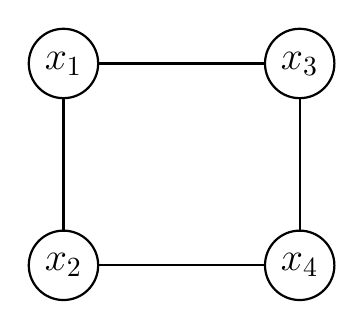
\begin{tikzpicture}[auto, node distance=3cm, every loop/.style={},
                    thick,main node/.style={circle,draw,font=\sffamily\Large\bfseries}]

  \node[main node] (1) {$x_1$};
  \node[main node] (2) [below =60] {$x_2$};
  \node[main node] (3) [right of=1] {$x_3$};
  \node[main node] (4) [right of=2] {$x_4$};

  \path[every node/.style={font=\sffamily\small}]
    (1) edge node [] {} (3)
    	edge node [] {} (2)
    (4) edge node [] {} (3)
    	edge node [] {}(2);
\end{tikzpicture}
\end{figure}
\begin{enumerate}
\examproblempart{To conduct MAP inference on this graph using exhaustive search, how many configurations must be checked?\\}
\bookletskip{0.2}

\framebox[14.7cm][l]{
	\begin{minipage}[b]{14.7cm}
	\inbooklet{Your answer: \MRFStudSolAA}
  
 	\solution{\MRFSolAA}
	\end{minipage}
 }
 
\examproblempart{Can MAP inference be run on this graph using a dynamic programming algorithm? Why or why not?\\}
\bookletskip{0.2}

\framebox[14.7cm][l]{
 	\begin{minipage}[b]{14.7cm}
 	\inbooklet{Your answer: \MRFStudSolAA}
  
 	\solution{\MRFSolAB}
 	\end{minipage}
 }
 \examproblempart{To run MAP inference on this graph using loopy belief propagation, how many messages must be computed?\\}
\bookletskip{0.2}

\framebox[14.7cm][l]{
 	\begin{minipage}[b]{14.7cm}
 	\inbooklet{Your answer: \MRFStudSolAC}
  
 	\solution{\MRFSolAC}
 	\end{minipage}
 }
 
\end{enumerate}

\examproblem{7}{ILP Inference formulation in Discrete Markov Random Fields}\\
\begin{enumerate}
\examproblempart{Suppose we have two variables $x_1\in\{0,1\}$ and $x_2\in\{0, 1\}$ and their local evidence functions $\theta_1(x_1)$ and $\theta_2(x_2)$ as well as a pairwise function $\theta_{1,2}(x_1,x_2)$. Using this setup, inference solves $\arg\max_{x_1,x_2} \theta_1(x_1) + \theta_2(x_2) + \theta_{1,2}(x_1,x_2)$. Using
\begin{align*}
\theta_1(x_1) &= \left\{\begin{array}{ll}1&\text{if~} x_1 = 0\\2&\text{otherwise}\end{array}\right. \quad
\theta_2(x_2) = \left\{\begin{array}{ll}1&\text{if~} x_2 = 0\\2&\text{otherwise}\end{array}\right. \\
\theta_{1,2}(x_1,x_2) &= \left\{\begin{array}{ll}-1& \text{otherwise}\\2&\text{if~}x_1 = 0 \text{~\&~} x_2 = 1\end{array}\right.
\end{align*}
what is the integer linear programming formulation of the inference task? Make the cost function and constraints explicit for the given problem, i.e., do not use a general formulation.

}
\bookletskip{0.2}   %in inches

% Solution box 
  \framebox[14.7cm][l]{
 \begin{minipage}[b]{14.7cm}
 \inbooklet{Your answer: \MRFStudSolBA}
  
 \solution{\MRFSolBA}
 \end{minipage}
 }

% Subproblem description
\examproblempart{What is the solution (value and argument) to the program in part (a). \\}
\bookletskip{0.2}   %in inches

% Solution box 
  \framebox[14.7cm][l]{
 \begin{minipage}[b]{14.7cm}
 \inbooklet{Your answer: \MRFStudSolBB}
  
 \solution{\MRFSolBB}
 \end{minipage}
 }

% Subproblem description 
 \examproblempart{Why do we typically not use the integer linear program for reasonably sized MRFs?
 }
 \bookletskip{0.2}   %in inches


% Solution box 
  \framebox[14.7cm][l]{
 \begin{minipage}[b]{14.7cm}
 \inbooklet{Your answer:  \MRFStudSolBC}
 
\solution{\MRFSolBC}
 \end{minipage}
 }
\end{enumerate}

\bookletpage
%%%%%%%%%%%% END OF PROBLEMS LIST
\end{enumerate}
\end{document}